


\chapter{A First Look at the Usability of Bitcoin Key Management}

\setchapterpreamble{\begin{quote} This chapter is adapted from published work supervised by Jeremy Clark and co-authored by David Barrera and Elizabeth Stobert ~\cite{eskandari2015first} \end{quote}}
% = = = = = = = = = = = = = = = = = = = = = = = = = = = = = = = = = = = = = = = = = =

\section{Introductory Remarks}

In all of the excitement surrounding Bitcoin, it is easy to forget that the decentralized currency assumes a solution to the longstanding problem of usable public key cryptography for user authentication. Studies of the usability of key management~\cite{GM05,GMSN+05,SBKH06,GFF06} have shown that there are numerous usability issues that prevent public key cryptography from being effectively leveraged by end users. Managing, controlling, and using cryptographic keys are complex tasks, and no clear solution has been proposed.  

Despite the known complexity in creating and managing cryptographic keys, the Bitcoin network and software clients use such keys extensively for many operations. For example, digital signatures, which require the Bitcoin software to read private keys into memory, are used to assert ownership over a specific set of Bitcoins. Thus, managing the same coins on multiple devices (\eg a desktop and a phone) requires the corresponding private keys to be copied to and made accessible on these devices. 

%\subsection{Consumer Protection} 

The consequences of losing exclusive control over an account containing monetary value connects the threat of losing a Bitcoin private key to that of losing an online banking password. However, consumers in many countries are legally protected from any liability of banking credential loss. Furthermore, most bank transactions are traceable and reversible, making it difficult to extract value from stolen banking credentials (most techniques involve a mule~\cite{FH12}). Bitcoin transactions are also traceable, however they are not reversible. Stolen Bitcoins can thus not be centrally or automatically recovered. Bitcoin users typically have no legal protection against loss or theft, and while stolen Bitcoins could be traced as they change ownership,\footnote{Public keys associated with specific Bitcoins are publicly available in the Bitcoin blockchain, but the identities of users who control those keys are not.} several mechanisms exist for laundering Bitcoins and similar digital currencies~\cite{MGGR13,BNMC+14}.

In an effort to address some of the complexities of key management, developers of Bitcoin software have created a variety of innovative technologies ranging from password-derived keys to air-gapped computers to physical printouts of private keys in the form of 2D barcodes. However, since none of these proposals have been evaluated in the Bitcoin context, it remains unclear which techniques have usability advantages.

For Bitcoin to flourish, adoption must expand beyond developers and tech-savvy enthusiasts to novice users. Expansion solidifies the need for a usable, comprehensible approach to Bitcoin. If users cannot safely manage Bitcoin keys, it may result in the users' loss of funds and/or a poor reputation for Bitcoin, both of which could dissuade further user adoption. 

In this paper, we aim to investigate the usability challenges surrounding key management in Bitcoin. To do this, we survey and categorize the most prominent Bitcoin key management proposals. Next we conduct an expert usability inspection technique known as a cognitive walkthrough~\cite{WRLP94} on popular examples of each proposal. Our goal is to identify overarching usability issues as well as advantages of specific proposals, allowing us to propose design recommendations for future Bitcoin clients.

%Despite decades of research on this exact issue in parallel technologies, such as digitally signed email, Bitcoin software technologies for creating, storing, and managing keys stall on many of the same basic issues. 

%At the same time, the developer-heavy Bitcoin community has been very prolific in producing deployed technologies with a wide variety of approaches to solving the challenges of a key-based system. We therefore argue that studying this suite of technology offers the clearest picture yet of the challenges in usable key management for digital signatures. 

Specifically, the contributions of the paper are as follows:

\begin{compactlist}
\item We perform a broad survey of six Bitcoin key management techniques which cover the vast majority of deployed Bitcoin software. 

\item Using the results from our survey, we propose an evaluation and comparison framework for Bitcoin key management techniques. The framework is based on 10 security, usability and deployability criteria, and enables direct comparison of current and future key management proposals. Using our framework we find that certain properties, such as trust in a central party enable additional beneficial properties. We also find that the disadvantages of certain properties, such as malware protection, outweigh the relative benefits.

\item We perform a cognitive walkthrough of six distinct Bitcoin clients and tools to identify usability issues while performing basic Bitcoin tasks (\eg viewing account balance, sending funds, \etc). We find that the metaphors and abstractions used in the surveyed clients are subject to misinterpretations, and that the clients do not do enough to support their users.

\end{compactlist}

%Our contribution is two-fold. First, the breadth of techniques that have been deployed for Bitcoin key management---from air gapped computers to paper printouts of QR codes to password-derived keys---demands an equally broad benchmark for objectively rating and comparing solutions. To address this, we develop an evaluation framework for Bitcoin key management techniques, based on the framework of Bonneau \etal~\cite{BHOS12}, to enable direct comparison between the various proposed solutions on usability, deployability and security criteria.

%Second, we perform cognitive walkthroughs focusing on the usability of six distinct Bitcoin key management approaches. Evaluating any set of competing approaches is difficult to do in a thorough, objective way without employing a formal usability evaluation. While user studies are considered the gold standard for this purpose, user studies have been traditionally employed to rigorously compare a small number of systems according to a narrow set of measurable properties. By contrast, we are interested in revealing broader mental model issues across a wider spectrum of tools. Expert evaluation enables the breadth of evaluation we require, and we use the cognitive walkthrough methodology to maintain rigour and objectivity in our evaluation. 

% \paragraph{Scope}
% The focus of this work is the configuration and management of the cryptographic keys required to hold and spend Bitcoin. This paper is not a study of the usability of Bitcoin itself---\eg sending and receiving transactions with various software tools. There is no doubt that such a study would be a valuable contribution to the literature, however we believe key management is the harder, fundamental problem that ultimately cannot be addressed with better user interfaces or dialogues. Without a secure, usable path-forward, we expect Bitcoin adoption among non-experts to stall.

%Bitcoin can be split into 3 parts: buying bitcoins (involving exchanges, OTC, etc), holding bitcoins (involving wallets, keys, etc), and spending bitcoins (creating transactions, waiting for verifications, etc). this paper focuses on the middle point. 

% = = = = = = = = = = = = = = = = = = = = = = = = = = = = = = = = = = = = = = = = = =
This chapter is a longer version of the published paper ~\cite{eskandari2015first}.

\section{Background}
\subsection{Bitcoin}
One subtlety of Bitcoin's transaction architecture is that in order to spend Bitcoins, the entire value of unspent outputs (\ie from previous transactions) must be spent. To accommodate this, Bitcoin clients automatically spend the full amount of unspent outputs and create multiple components in the transaction: one component will send part of the unspent coins to the intended recipient, and the other component will send the remaining inputs back to the sender as \emph{change}. It is technically possible (and some clients behave this way) to send change back to the sending address. However, to enhance anonymity, the reference client generates fresh addresses (and corresponding private keys) to receive the remaining transaction amount. 

As more transactions are made, Bitcoin clients must keep track of multiple private keys for use in future transactions. Many clients prominently display a Bitcoin balance on the main screen, which represents the sum of all unspent outputs for which private keys are available. 

One subtlety of Bitcoin transactions is that each XBT amount in the set of inputs must reference past transactions where the address received adequate XBT to cover the input amount. The complexity here is that a transaction must completely spend the amount received in these past transactions even if it is larger than the amount in the current transaction. To enable this, transactions will output the surplus XBT back to the sender as `change.' Change can be sent back to the same input address, or to enhance privacy, it can be sent to a brand new address created by the sender's client (called `change addresses'). 

\subsection{Usability of Key Management}

Passwords remain the most common form of user authentication~\cite{Herley.2012}. Private key-based authentication is rarely used by non-experts, and is typically never used as the default configuration in applications which support this authentication method. Transport Layer Security (TLS) client-side certificates have failed to reached wide-spread deployment. Secure shell (SSH) uses passwords by default, and recent efforts to reintegrate them in a different form (\eg origin-bound certificates~\cite{DCBW12}) still rely on passwords as the primary authentication mechanism.


Password managers, when configured to generate or store system-chosen random passwords, share at least one property of cryptographic keys: such passwords become something you \emph{have} instead of \emph{know}. However, if access to such a password is lost, online services generally offer account recovery mechanisms (\eg based on email). No such recovery mechanism exists for self-managed cryptographic keys.

The use of public key systems by non-experts that is closest to Bitcoin is arguably encrypted/authenticated email, in particular Pretty Good Privacy (PGP) and its open-source alternatives (\ie GPG and OpenPGP). Beginning with \emph{Why Johnny Can't Encrypt}~\cite{WT99}, the usability of public key technology has been well-studied from a usability perspective~\cite{GM05,GMSN+05,SBKH06,GFF06}. The findings of this literature are diverse but relevant observations include the following: (1) the metaphor and terminology behind public and private keys is confusing; (2) it is difficult to correctly obtain other users' public keys; (3) key migration between devices is difficult. This literature tends to focus primarily on encryption and not signatures, but we find some overlap to the work presented here \footnote{``Why King George III can encrypt,'' \textit{Freedom to Tinker} (blog), 6/6/2014.}.

% = = = = = = = = = = = = = = = = = = = = = = = = = = = = = = = = = = = = = = = = = =

\section{Bitcoin Key Management Approaches} 
\label{sec:approaches}

Before turning to a detailed usability evaluation, we evaluate from a systems perspective each category of tool for managing Bitcoin private keys. We highlight security and deployability issues, and note relevant details of the Bitcoin protocol that create complexities and potential discrepancies with users' mental models.

\subsection{Keys in Local Storage}
\label{sec:localstorage}
One way in which Bitcoin software manages several private keys is by storing these keys on the device's local storage, typically in a file or database in a pre-configured file system path. When a new transaction is created, the Bitcoin client can read the keys and immediately (possibly without any further user input) broadcast the transaction over the network. The reference Bitcoin client (Bitcoin Core), as well as certain mobile wallets (\eg Android Bitcoin Wallet) use this approach, storing private keys in a file (referred to as a \emph{wallet}) inside the user's home or application directory. 

%advantages
Storing keys in a locally accessible file has several advantages. First, there is no additional cognitive load on users, since only the software must access the file. Second, a practically unlimited number of keys can be stored on disk due to the small size of keys. Third, the Bitcoin software can automatically generate keys and create transactions without additional input or actions from the user. 

%threats-malware
Storing keys locally also creates several threats, which the user must consider. For example, the file storing private keys can be read by any application with access to the user's application folder. Malware authors may be particularly interested in exploiting this key management approach, since access to the local file results in the adversary gaining immediate access to the victim's funds. One of the first examples of private key-stealing malware was discovered by Symantec in 2011~\cite{coinbit}, with many other similar malware examples following suit.

%sharing or losing
Users must be cautious to not inadvertently share their Bitcoin application folder (\eg through peer-to-peer file sharing networks, off-site backups or on a shared network drive). Physical theft, especially in the case of portable computers or smartphones must also be considered. Similar to the storage of other sensitive files, threats to digital preservation~\cite{BKM05} should be taken into account. Examples include general equipment failure due to natural disasters and electrical failures; acts of war; mistaken erasure (\eg formatting the wrong drive or deleting the wrong folder); bit rot (\ie undetected storage failure); and possibly others. If storing private keys for a long period of time (\eg a trust fund or long-term savings), users must also preserve a specification of the file format to ensure the keys can continue to be read.

%key churn
The reference Bitcoin client pre-generates keys in a batch of 100 (these keys are known as the keypool). When a transaction is made, the next available key is selected from the keypool for receiving change. The keypool is then periodically refilled with a new batch of keys as necessary. This \emph{key churn} requires users to periodically create new backups of their key storage file to ensure that new keypool keys are stored. 

The user must also be wary of \textit{key churn} as the \bitcoinclient client sends change to new addresses. By default, it creates private keys in batches of 100 (called a keypool). This has the unfortunate side-effect that backups become obsolete after the user churns through their current keypool. The user interface of \bitcoinclient does not display change addresses or give any indication that they are being used, and so it is quite natural that a novice users' mental model will not account for this behaviour, and they will not act accordingly to ensure they re-backup \walletfile each time they deplete the keypool (another event that is not communicated to the user in any way). To address key churn, alternative Bitcoin clients return all change to the same address or derive all change addresses, called a \textit{deterministic wallet}, from a single key.

Another disadvantage of using \bitcoinclient is that it requires a copy of the entire blockchain to validate the balance associated with each of the keys it will create. At the time of writing, the blockchain is 35 GB.\footnote{\url{https://blockchain.info/charts/blocks-size}} For a new installation, it is not uncommon for it to take days to obtain a local copy of blockchain from the Bitcoin peer-to-peer network.

% \paragraph{Mobile Wallets} A number of mobile wallets for OSes like Android and BlackBerry have been proposed, including Bitcoin-wallet\footnote{\url{https://androidobservatory.org/app/9A33CF64239CC26F6E52F80BE83AF39B93F261C0}} and Mycelium.\footnote{\url{http://mycelium.com}} The main challenge for mobile platforms is the general unfeasibility of obtaining and storing the entire blockchain. Instead, they implement a `thin client' approach which shortcuts full validation of the blockchain by placing bounded trust in the Bitcoin peer-to-peer network (specifically, it uses a protocol called simplified payment verification or SPV~\cite{Nak08}). SPV is also used on some desktop clients. Regarding key management, mobile clients are not much different from \bitcoinclient and still store keys in a local file on the device that is subject to the same threats: unauthorized access and non-preservation.

\subsection{Password-protected (Encrypted) Wallets}
Certain Bitcoin clients allow a locally stored wallet file to be encrypted with a key derived from a user-chosen password or passphrase. 
%A common approach is to use the well known password-based key derivation function (PBKDF2~\cite{pbkdf2}). 
Password-protected wallets appear to address only \emph{physical} theft of the underlying storage device, requiring brute-force of the password if the file containing private keys is stolen. Password protection seems less useful in the case of \emph{digital} theft; if malware can be installed on to the device storing the wallet, it is reasonable to assume a keystroke-logging module would be present, limiting or nullifying the benefits of the password protection.

% At the time of our analysis, this was possible but not the default in \bitcoinclient, however it is enabled by default in Multibit\footnote{\url{https://www.multibit.org}}, another popular desktop client. 
Password-protected wallets share the advantages and disadvantages of non-encrypted wallets (see Section~\ref{sec:localstorage}), with a few subtle differences. Password-protected wallets trade recoverability and usability for the mitigation of physical theft. If the password is forgotten, users lose the balance of their password-protected wallet since no mechanism exists for recovery\footnote{Of course, exhaustive search of the password space is theoretically possible, and is available as a service: \url{http://www.walletrecoveryservices.com}}. For day-to-day use, users must unlock the wallet by entering their password when new transactions are made. 

The trade-off of a password-protected wallet is that users can lose their XBT by forgetting the password protecting their wallet. No recovery mechanism exists (as this mechanism could itself be exploited in the case of theft) short of exhaustive search, which is an available service.\footnote{\url{http://www.walletrecoveryservices.com}}

Password-protected wallets may mislead the user to believe that the password itself provides access to their funds regardless of the location of the device storing the wallet, as would be congruent with a traditional mental model for web-based online banking. Users may be surprised to discover that they cannot access their funds at a new device by simply entering their encryption password; the wallet file must also be transferred to the new device. 

\subsection{Offline Storage of Keys}
\label{sec:offline storage}
To further protect Bitcoin private keys from malware-based threats, wallets can be stored offline on some form of portable media, such as a USB thumbdrive. Keeping keys offline enables the use of traditional physical security techniques (\eg storing the drive in a fire-proof safe) to protect the wallet. However, offline storage has the drawback of making the wallet inaccessible for immediate use by software, preventing users from spending funds unless the offline storage media is nearby. As expected, offline storage can be used for backup, but all copies of the wallet must be kept offline for the full benefits of theft-protection to be realized. Prior to offline storage (wallet creation) and after storage (future transactions), the wallet will be exposed on a computational device, potentially to malware. 

\begin{figure}[htb]
  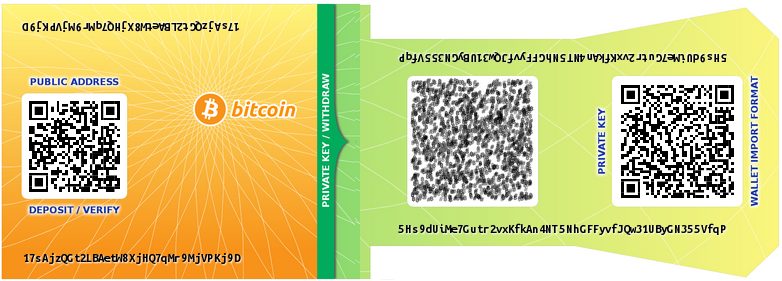
\includegraphics[width=\linewidth]{fig/paperwallet.png}
  %\caption{Bitcoin paper wallet generated using \url{https://bitcoinpaperwallet.com}. The printout is designed to be folded such that the private key (right) remains hidden while the public component (left) remains visible.}
  \label{fig:paperwallet}
\end{figure}

An interesting case of offline key storage is paper wallets (see ~\autoref{fig:paperwallet})
%\footnote{\url {https://bitcoinpaperwallet.com}}\
where private keys are printed onto paper typically in the form of a 2D barcode (\eg a QR code) or as a long sequence of characters. Barcodes facilitate reading the key back into a Bitcoin client by, for example, scanning the code with a smartphone camera. Securing a paper wallet is similar to securing cash, which most users should be comfortable with. However, funds can be stolen from a paper wallet by simply observing the QR code (\eg on live television\footnote{``A Bloomberg TV Host Gifted Bitcoin On Air And It Immediately Got Stolen,'' \textit{Business Insider}, 10/23/2013.}), which is not possible with physical money. Thus transporting a paper wallet securely requires that the printed contents remain unobservable at all times.  Users must remember that a paper wallet does not contain the funds itself, but rather enables signing authority over a set of Bitcoins. For example, if a paper wallet is discarded after funds are spent, the paper wallet still provides access to any future funds that may be sent to that address.\footnote{``Five Ways to Lose Money with Bitcoin Change Addresses,'' \textit{Bitzuma} (Blog), 17/03/2014.} 

Finally, users still need to be cautious of key churn and that spending XBT from a paper wallet does not result in XBT being sent to a change address not included in the paper wallet. 

As with any long-term storage, users must preserve software capable of decoding the QR code in the event that the paper wallet generation service is unavailable when attempting to reload keys onto a device. As of writing, many Bitcoin clients as well as offline storage solution use a common ``wallet import format'', which involves manipulating an ECDSA private key by performing cryptographic hashes, adding a checksum for integrity, and encoding the resulting string into Base58.\footnote{Base58 avoids the use of characters such as ``0, O, I, and l'' which may look visually similar, and also avoids punctuation characters which may trigger software (\eg e-mail clients) to perform line breaks.}

\subsection{Air-gapped Key Storage}
In offline storage, we assume the device or media holding private keys cannot perform computations such as creating digital signatures. We distinguish this type of storage from air-gapped storage, where wallets are stored on a secondary device that generates, signs, and exports transactions, but this secondary device is never connected to a network. When spending Bitcoins using an air-gapped device, a transaction is created from the air-gapped device and the resulting signed output transported (usually through portable media) to an Internet-enabled device for transmission onto the Bitcoin network. 
%A notable client supporting this setup is Armory.\footnote{\url{https://bitcoinarmory.com}} 

An air gap improves theft-resistance by never directly using a private key on an Internet-connected device. However, air gapped devices are capable of actually executing malware if infected. Malware may jump the air gap by infecting the portable media used to export signed transactions.

While not literally an air gap, hardware security modules (HSMs) emulate the properties of an air gap by isolating the key material from the host device, and only exposing the ability to sign transactions. Bitcoin-specific HSMs are under active development at the time of writing and a few have been recently released (\eg Trezor\footnote{\url{http://www.bitcointrezor.com}}).

Note that the consequences of obtaining access to the private keys are not much different from accessing a transaction-signing oracle for the wallet---both allow the current balance of Bitcoin to be stolen. However, future funds may be protected if access to the signing oracle is non-persistent. 

\subsection{Password-derived Keys} 
Thus far, all key management solutions have required users to maintain cryptographic keys. The remaining two solutions enable users to access their Bitcoin with a password instead. 

The first approach is to derive cryptographic keys from a user-chosen password (\eg using PBKDF2~\cite{pbkdf2}, manipulating the output to produce a valid Bitcoin private key). The disadvantage of using this approach directly is that only one resulting keypair is created, requiring the user to select a new (different) password for a new keypair. 

A more robust approach is described in the Bitcoin Improvement Proposal 32~\cite{bip32}, and is known as a Hierarchical Deterministic (HD) Wallet. HD wallets deterministically derive a set of private keys from a master secret (a randomly chosen passphrase). These keys can derive new private keys. The deterministic nature allows the password holder to view the balance, as well as spend the funds, of any sub-account derived from the password. However, if the private key on one of the sub-accounts is compromised, only the funds sent to that sub-key (or sub-keys derived from it) may be stolen. 

% applied to the password and expand the seed into the required number of keys with a PRG. Thus it is a special case of a deterministic wallet, where the initial seed is password-derived instead of randomly chosen. A notable tool here is Brainwallet.\footnote{\url{http://brainwallet.org/}}

Password-derived wallets are targeted at loss-prevention and simpler cross-device access. The challenges of preserving access to a digital file are no longer necessary as long as the wallet can be re-generated from a memorized password. The primary drawback of a password-derived wallet is that weak user-chosen passwords can be found through unthrottled exhaustive search since a fingerprint of the associated public key will be in the global public ledger if the account holds any amount of Bitcoin. Rainbow tables~\cite{oechslin2003making} for password-derived keys have been developed.\footnote{D. Martyn. ``Bitcoin `Brainwallets' and why they are a bad idea,'' \textit{Insecurety Research \emph{(sic)}} (Blog), 26 Mar 2013.} Finally, it remains unclear whether memorization poses an advantage over maintaining a digital file when preventing loss---a forgotten password will orphan all funds in the account.


\subsection{Hosted Wallets} 
A final approach to key management is to host user accounts on a third-party web service. In this case, the service maintains possession of the private keys. Hosted wallet web services provide the user with access to transactional functionalities through standard web authentication mechanisms, such as a password or two-factor authentication, and may also offer password recovery mechanisms. Bitcoin smartphone applications that act as clients to hosted wallets benefit from reduced application complexity (\ie no need to perform cryptographic operations on the device) and brick and mortar bank-like user interfaces. Currency exchange services that allow Bitcoin to be exchanged with fiat currency effectively provide this service, as do web services deployed specifically to host wallets.

The popularity of hosted wallets appears to be justified, since these services provide the closest experience to traditional online banking. However, their use has also been hampered by high profile breaches and fraud. Users' funds have been unrecovered from services such as Mt.Gox and Bitcoinica, while popular exchanges such as BTC-E have suffered losses but fully reimbursed users. Thefts and losses from/by third party services are catalogued online\footnote{https://bitcointalk.org/index.php?topic=576337.0} and include over 40 events involving losses greater than 1000 XBT.\footnote{At the time of writing, 1000 XBT > 650\,000 USD.}

%proofs of solvency?
It is natural to expect hosted wallet services will become primary targets of attack since these services typically hold large amounts of Bitcoin. Offloading the task of key management to a third-party requires users to assume the risk that the service could be breached and funds lost, in exchange for a traditional online banking-style user experience. 

As a counter-measure to theft, hosted wallet providers often keep only a small float of their holdings online (called \textit{hot storage}) and store the majority of their holdings offline in \textit{cold storage}. This has the drawback of causing delays in transactions for users if the hot storage amount is exhausted.
%and is still susceptible if hot storage theft goes undetected as the float will be persistently replenished. 
Hosted wallet services may also allow audits, where they cryptographically prove possession of sufficient Bitcoin to match their liabilities.  
%to demonstrate that they are not covering up any missing XBT (which would not necessarily be immediately apparent---\cf \fixme{a fractional reserve)}.  

Another approach that falls under the hosted wallet category is a hybrid hosted wallet. Hybrid wallets use client side encryption (typically in Javascript) to encrypt all private keys and sensitive data. The web service is then only used for broadcasting transactions to the network and for displaying the user's balance (which requires inspecting the entire blockchain).

Other than server side encryption and security measures, It uses client side encryption (javascript) to encrypt all the private keys and sensitive data with user's password and sends the encrypted data as a random base64 string to the server. With this implementation, there is no access to the private keys and the final balance from anyone whom have access to the server's data \footnote{\url{http://bitcoin.stackexchange.com/questions/5249/how-secure-is-blockchain-info}}. Blockchain.info uses this implementation for its hosted wallet.

% = = = = = = = = = = = = = = = = = = = = = = = = = = = = = = = = = = = = = = = = = =


\begin{sidewaystable*} %[ht!] 

\renewcommand{\arraystretch}{1}
\centering
\begin{tabular*}{0.9\textwidth}{@{\extracolsep{\fill}} llccccccccccccc}

\textit{Category} &
\textit{Example} & 
\headrow{Malware Resistant} & %Part if malware crosses air gap. Malware: theft? what about DoS? Ransomware
\headrow{Key(s) Kept Offline} &  %Part if one of two factors are offline
\headrow{No Trusted Third Party} &
\headrow{Resistant to Physical Theft} &
\headrow{Resistant to Physical Observation} &
\headrow{Resilient to Password Loss} & %Part if resettable by TTP
\headrow{Resilient to Key Churn} &
\headrow{Immediate Access to Funds} &
\headrow{No New User Software} & %Beyond a browser and the default client
\headrow{Cross-device Portability} & 
\headrow{ } & % Something about format decay
\headrow{ } \\ \hline 

Keys in Local Storage & \bitcoinclient	&	&	&\full	&	&\full	&\full	&\full	&\full	&	&	&&\\
Password-protected Wallets &\multibit	&	&\prt	&\full	&\prt	&\full	&	&\full	&\full	&	&	&&\\
Offline Storage	&\paper				&\prt	&\full	&\full	&	&	&\full	&	&	&	&\full	&&\\ 
Air-gapped Storage & \armory 		&\prt	&\full	&\full	&	&\full	&\full	&\full	&	&	&	&&\\
Password-derived Keys & \brain		&	&\full	&\full	&\prt	&	&	&\full	&\full	&\full	&\full	&&\\ 
Hosted Wallet (Hot) & \coinbase			&	&	&	&	&	&\full	&\full	&\full	&\full	&\full	&&\\ 
Hosted Wallet (Cold)	&				&\prt	&\full	&	&	&	&\full	&\full	&	&\full	&\full	&&\\
Hosted Wallet (Hybrid)	&	\block			&	&\prt	&\prt	&	&	&\full	&\full	&\full	&\full	&\full	&&\\\hline
Cash &							&\full	&\full	&\full	&	&\full	&\full	&\full	&\full	&\full	&\full	&&\\ 
Online Banking &					&	&	&	&	&	&\full	&\full	&\full	&\full	&\full	&&\\ \hline 
																			
\end{tabular*}

\caption{A comparison of key management techniques for Bitcoin (contrasted with traditional financial services). \full~ indicates the category of client is awarded the benefit in the corresponding column. \prt~partially awards the benefit. Details provided inline.}
\label{tab:prims}
\end{sidewaystable*}
  

\section{Evaluation Framework}
% In this paper, we evaluated different approaches to key management in Bitcoin from both a systems perspective and a usability persecutive. On the usability side, in particular, some findings are very specific to the exact design of the software evaluated and its interfaces. Other usability issues are more fundamental to the category of key management the particular tool falls under. 
In this section, we systematize the major category-wide issues we have uncovered in describing the various key management approaches used by Bitcoin clients. We present an evaluation framework based on 10 criteria as shown in Table~\ref{tab:prims} and discussed in the following subsections. This framework both summarizes the advantages and disadvantages of the various approaches we have evaluated, while also providing a benchmark for evaluating future key management proposals. The framework is adapted from a similar framework for evaluating password replacement schemes~\cite{BHOS12}.

\subsection{Evaluation Criteria}
We briefly enumerate the criteria used to evaluate each proposal in the framework below. 

\paragraph{Malware Resistant}
\label{Malware Resistant}
Malware designed to steal Bitcoin wallets and related passwords has been observed in the wild. Wallets that are not stored on an Internet-connected device, or devices capable of performing computations are considered malware resistant (\full), unless creating a transaction involves transferring to a computational device (\prt). 

\paragraph{Key Stored Offline}
\label{Key Kept Offline}
For archival storage of infrequently used keys, keys not directly accessible from an Internet-connected device---either due to being offline (\full) or online but password-protected (\prt)---are preferable. 
%(For traditional banking online, we interpret this benefit as authority over the account being kept offline, which it is not).

\paragraph{No Trusted Third Party}
\label{No Trusted Third Party}
All Bitcoin key management tools are trusted to a certain extent. 
%Even an open source Bitcoin client might contain an undiscovered backdoor that kleptographicly steals high value private keys. 
This criteria considers the absence of a persistent trusted third party (\full) that maintains direct signing authority over a user's Bitcoin. 

\paragraph{Resistant to Physical Theft}
\label{Resistant to Physical Theft}
If the cryptographic keys are stored on some media or device that can be physically stolen, we do not consider the tool to be resistant to physical theft. Within our framework, the only tools meeting this requirement rely on a human memorized password being necessary for key recovery. These are awarded (\prt) since passwords tend to be weak and may not adequately resist unthrottled guessing. 

\paragraph{Resistant to Physical Observation}
\label{Resistant to Physical Observation}
Physical observation, such as observing key strokes or capturing QR codes with a camera, may result in access to a user's Bitcoin account. 

\paragraph{Resilient to Password Loss}
\label{Resilient to Password Loss}
% NOTE: I changed the first score from (\full ~ if not) to (\prt), but it's somehow unclear and might need further explanation
If passwords are used (\prt), the loss of a password could result in some Bitcoin becoming unrecoverable if it is a necessary authentication factor in obtaining access to the signing key. For solutions where funds are held by third parties, these entities could provide a password recovery/reset mechanism (\full).

\paragraph{Resilient to Key Churn}
\label{Compatible with Change Keys}
Assuming the client sends change from transactions to a newly created change addresses, a tool is resilient to key churn if it can maintain access to the funds even after exhausting the initial keypool (\full). Tools not awarded this benefit are not guaranteed to maintain persistent access to new change addresses, and any balance sent to these addresses may be lost.

\paragraph{Immediate Access}
\label{Immediate Access}
Key management mechanisms that maintain direct access to the wallet enable Bitcoin to be transacted immediately (\full). We award this benefit to techniques that require a user to enter a password. We omit the benefit for techniques that require data to be obtained from external storage medium or secondary device. 

\paragraph{No New User Software}
\label{No New Software}
Some approaches require users to install new software on their system, for which the user may not have suitable permission, or software may not be developed for their specific platform (\eg some mobile platforms). By contrast, some tools can be executed from widely available software such as any standards-compliant web browser (\full). 

\paragraph{Cross-Device Portability}
\label{Portable}
A key management technique is cross-device portable (\full) if it allows easy sharing of the a Bitcoin address across multiple devices with minimal configuration or usability issues due to complexities like key churn.

\subsection{Discussion}
\autoref{tab:prims} demonstrates that key management approaches provide varying levels of security and convenience, with no single approach being obviously superior to others. One possible takeaway from our evaluation and comparison is that users can benefit heavily by offloading key management to a trusted party (\eg hosted wallets). The lower right side of the chart focuses on usability properties that are already present in traditional financial services (\ie resilient to password loss, no new software, cross-device portability). These properties are difficult to obtain if users independently manage their keys through one of the local storage techniques. Of course, the disadvantage of trusting a third party is that Bitcoin funds are now bound by a contractual agreement between users and the hosted wallet provider, negating one of the primary features of Bitcoin: a fully decentralized currency. Users in countries lacking regulatory maturity for digital currencies should exercise caution when trusting a third party with large amounts of Bitcoin. 

Based on our analysis, users can be given the concrete advice of treating digital currency much like they would treat fiat currency: keeping small amounts in ready-to-spend form (\eg local storage or online hosted walled) mimicking cash, and keeping larger sums in more difficult to access but more secure storage (\eg air-gapped or offline storage) mimicking a savings account or trust fund. Barber \etal~\cite{Barber2012} suggest the use of ``super wallets'' where users essentially run their own personal bank. A super-wallet keeps keys across multiple devices and requires all (or a subset using a threshold scheme) to be present to transfer funds to sub-wallets. Pre-configured transfers of small amounts can be authorized to move funds to sub-wallets that can be used for day-to-day spending. While the idea of super-wallets is intuitive, the implementation of such a scheme could introduce high levels of complexity. 



% , no one tool provides a clearly beneficial set of properties over another. We also note that the approaches are not necessarily mutually exclusive. One tool may be used for a small float of XBT, while longer term savings may utilize a different mechanism. The hosted wallet solution provides essentially the same set of properties as online banking---what it lacks is regulatory maturity, consumer protection, and established businesses with track records that earn the trust (encapsulated by the trusted third party criteria) instilled in them. Of all the solutions, further development in hosted wallets seems the most promising for further Bitcoin adoption, primarily among novice users.

% = = = = = = = = = = = = = = = = = = = = = = = = = = = = = = = = = = = = = = = = = =

\section{Usability Evaluation of Bitcoin Clients}

\subsection{Methodology}

We used a series of cognitive walkthroughs~\cite{WRLP94} to evaluate the usability of six Bitcoin clients. Cognitive walkthrough is a form of expert evaluation where an expert (or group of experts) steps through the design to evaluate aspects of its usability. The focus of the walkthrough is on the novice user and emphasizes \emph{learnability}. At each step, the evaluators ask three questions: Will the user see what to do? Will the user see how to do it? And once it is done, will the user know if they have performed the correct action?

We chose to use cognitive walkthroughs for several reasons. First, it allowed us to choose and compare standard tasks on disparate tools, and gave us easily compared insight into the common problems and successes of different Bitcoin clients. The cognitive walkthrough also allowed us to keep the focus on the novice user. The goal of our evaluation was to uncover problems specific to key management within Bitcoin software rather than to evaluate the usability of the clients themselves.
%Gathering novice users of Bitcoin for a user study could potentially be quite difficult; Bitcoin is still comparatively uncommon, and many users are also Bitcoin enthusiasts, often with additional knowledge of cryptography or PKI. Bitcoin is only in the process of developing a base of novice users. \fixme{Elizabeth, can you add something here saying that our intention is not to be thorough, but rather see (1) if there are issues, and (2) if there are any themes in the issues.}

%citecheck: Not sure what to cite here...! maybe say something about being anecdotal??

A number of usability evaluation methodologies employ expert review. We use a cognitive walkthrough \cite{WRLP94}, which has been used previously to study closely-related subjects: public key technology~\cite{WT99} and software configuration~\cite{COA07}. A cognitive walkthrough is premised on the idea that users learn through exploration of the software, instead of reading manuals. They attempt to perform the task they want completed and rely on the interface to intuitively guide them through proper design, interface cues, and feedback. 

For our cognitive walkthrough, we defined a set of core tasks involving key management that a typical user needs to perform. We compared the results of each walkthrough against a standard set of evaluation guidelines, combining aspects of an heuristic evaluation~\cite{HeuristicEvaluation} with the walkthrough in order to interpret our results. 

Each of the following four tasks was independently performed by 2 experts to evaluate each tool:

\begin{compactlist}
	\item[\bf T1] Configure a new Bitcoin address and obtain its balance. This task involves launching the Bitcoin client (or logging into one if hosted online) for the first time. After a new address has been generated (either explicitly or transparently in the background), the user should be confident that the address' balance is XBT~0.00000000. The user should also be able to find their receiving Bitcoin address.\label{sec:ct-1}
	\item[\bf T2] Spend Bitcoin. Send some amount of Bitcoin to an arbitrary (but valid) Bitcoin address. This task requires the user to create a new transaction, entering relevant information such as recipient, amount, \etc\label{sec:ct-2}
	\item[\bf T3] Spend Bitcoin from the same address as above, but on a secondary device. This task may require copying private keys to the secondary device, entering passwords on multiple devices, or logging in to a hosted wallet provider on a different browser.\label{sec:ct-3}
	\item[\bf T4] Recover from the loss of the main credential. In the case of locally stored keys, this task involves restoring a file from backup. Otherwise this task involves recovering from password loss.\label{sec:ct-4}
\end{compactlist}

Since the focus of our walkthrough was on configuration and learnability, we used a set of heuristics first developed for a usability evaluation of Tor~\cite{COA07}. We chose to use these guidelines because like the anonymity software, successfully managing Bitcoin involves the application of complex cryptographic knowledge in an everyday activity. The set of guidelines, from~\cite{COA07}, are: 

%The literature contains a variety of evaluation guidelines or heuristics to use for expert review of security-related tools. We chose to use the guidelines proposed in a usability evaluation of configuring the anonymity software Tor~\cite{COA07} since we share a focus on configuration. 
%This set is itself culled from numerous sources in the literature~\cite{WRLP94,WT99,Cra03,KBK05,COB06}.


	
\begin{compactlist}
	\item[\bf G1] Users should be aware of the steps they have to perform to complete a core task.
	\item[\bf G2] Users should be able to determine how to perform these steps.
	\item[\bf G3] Users should know when they have successfully completed a core task.
	\item[\bf G4] Users should be able to recognize, diagnose, and recover from non-critical errors.
	\item[\bf G5] Users should not make dangerous errors from which they cannot recover.
	\item[\bf G6] Users should be comfortable with the terminology used in any interface dialogues or documentation.
	\item[\bf G7] Users should be sufficiently comfortable with the interface to continue using it.
	\item[\bf G8] Users should be aware of the application's status at all times.
\end{compactlist}


Cognitive walkthroughs are primarily relied on when the breadth of the evaluation makes a user or field study prohibitive to run due to time and cost. We examine six Bitcoin key managers, from configuration through transaction authorization through key recovery. If the results of the cognitive walkthrough narrows the field significantly, user studies are an appropriate follow-up for detailed examination of the most challenging set of tasks within one or two solutions. Thus while our result can be considered a first-pass at the problem, we felt the richness of the result merits sole presentation.

\subsection{Evaluated Clients}
Real-world evaluation of the general approaches detailed in \autoref{sec:approaches} is difficult. Thus, we select six distinct Bitcoin clients or utilities that implement the key management approaches described. For the purposes of our usability evaluation, each client was evaluated in its default configuration on OS X unless otherwise stated. 

\paragraph{Keys in Local Storage} The reference Bitcoin client, Bitcoin Core~\cite{bitcoinqt}, is a cross-platform client that stores keys locally (optionally encrypted with a password). Bitcoin Core is the first recommended client on the \url{bitcoin.org} website. 

\paragraph{Password-protected (Encrypted) Wallet} We use the MultiBit~\cite{multibit} client (also recommended on \url{bitcoin.org}) since it provides a more convenient way to encrypt with a user-chosen password.

\paragraph{Offline Storage} We use paper wallets as offline storage. While paper wallets can be as simple as printing private keys on to paper, we select the paper wallet creation website \url{Bitaddress.org}~\cite{bitaddress}. Bitaddress allows users to generate new randomized keys in their web browsers, and then print QR encoded keys. 

\paragraph{Air-gapped Storage} We select the Bitcoin Armory~\cite{bitcoinarmory} client which includes functionality for creating an offline wallet that can be used to sign and export transactions. 

\paragraph{Password-derived Keys} One of the simplest ways to create a password-derived key is on the Brainwallet~\cite{brainwallet} website. The site allows users to enter a passphrase which is converted into a private key. 

\paragraph{Hosted Wallets} We use \url{Blockchain.info}~\cite{blockchain} as our hosted wallet provider. As of writing, Blockchain.info advertises the management of over 2.5 million user wallets.

%===========================================================

\section{Results}

The following is the full details of our walkthroughs, which expands on the shorter version presented in the conference version of this paper.

\subsection{Keys in Local Storage (\bitcoinclient)}
We begin with an evaluation of \bitcoinclient, the original Bitcoin wallet client, which uses locally-stored keys. We assume the user has downloaded and installed the \bitcoinclient client (it has a straight forward wizard installation procedure).

\paragraph{T1: Configure} \bitcoinclient transparently generates a new set of addresses on first run, but shows no notification to the user that this has occurred (fails G3). The receiving address can be found under the \emph{Receive coins} tab, but this could be easily confused with the \emph{Addresses} tab which contains a contact list of other user addresses (fails G2). 

To retrieve the account balance, \bitcoinclient must be online and the user must wait until a full copy of the blockchain has been downloaded.  Except for a small status indicator on the bottom-right side of the window that shows a small red cross in-between two black windows, there are no other messages to show the user that the application should be online. Due to the size of the blockchain, this may take hours to days to complete. A status bar displaying ``Synchronizing with network'' shows the progress of the blockchain download (achieves G8), but the terminology may be too technical for novice users, With a mouse over the icon, it says `0 active connections to bitcoin network' which is likely unfamiliar language that does not help resolve the error (fails G4 and G6). Once the blockchain has been downloaded, the balance is displayed on the \emph{Overview} tab (achieves G3). 

\paragraph{T2: Spend} Spending Bitcoin is straightforward since the keys are readily available to the \bitcoinclient client. Users spend Bitcoin by navigating to the \emph{Spend} tab (achieves G1 and G2). Since our focus is on key management, we do not evaluate the actual completion of transactions (which may have additional usability issues). We focus on ensuring the key is available to the software tool (which is not so straightforward with \eg offline storage). 

\paragraph{T3: Spend from Secondary Device} Installing \bitcoinclient on a secondary device creates a new set of keys. Users may not understand that the keys must be copied to the secondary device (fails G1), and if so, what file must be copied (fails G2). The correct procedure is to back up the \walletfile with the `backup wallet...' option in the `File' tab of the first installation and chose a directory to save the \walletfile. Next the user must securely transfer this file to the secondary device, and no guidance is provided on how to do this (fails G2) or the dangers of transferring it through an insecure mechanism (fails G5).

Assuming the user has transferred \walletfile to the secondary device, she could try looking for import options in the newly installed wallet client, or drag and drop the \walletfile into the client, but she would fail to do so as no import option exists. The documentation is inadequate here as well---there is actually nothing in the help menu except a debug window that is for advance user to tweak the application (fails G2 and G6)!

The only mechanism to activate the wallet on a secondary file is to actually overwrite \walletfile on the secondary device with \walletfile from the first. It is unlikely any novice user would be able to complete this step. It is actually even difficult to find the path to copy \walletfile to on the new device---this could be possible by searching the local file system for \walletfile, which might not succeed due to non-searchable system reserved folders or not knowing the exact file name (spotlight does not return any result for \walletfile). More likely, the user will search online.\footnote{\url{https://en.bitcoin.it/wiki/Data_directory}} On OS X, the path is \texttt{/Users/User/Library/Application Support/Bitcoin/wallet.dat}.

The next step is to replace the new \walletfile with the one from the primary device. It should be noted that the name of the file should be exactly \walletfile for the \bitcoinclient to be able to read the file. Some of errors that the user might encounter during this procedure are:
\begin{itemize}
	\item The user might copy \walletfile from the primary device wallet client path instead of the one exported through the back up option. This could cause a corrupted \walletfile that is not readable by the secondary device's \bitcoinclient. This is due to \bitcoinclient's procedure to lock \walletfile while it is in use. The error is recoverable by repeating the process correctly (fails G4). 
	\item User should wait for the \bitcoinclient on the secondary device, to download and sync the Blockchain from the P2P network to be able to authorize a transaction.
	\item On the secondary device, the final balance might be wrong and there would be the need to resynchronize and rescan the blockchain to have the correct final balance (fails G3).
\end{itemize}

Finally, this process must be repeated if either client exhausts their keypool. If both do, there is no way to merge the new keys in the keypool, and replacing one \walletfile with the other will lead to unrecoverable funds (fails G5). 

We note that replacing the key file may require  a re-scan of the blockchain to display the correct balance (fails G3).

\paragraph{T4: Recovery} If only one device is used, there is no way to recover from loss of the key file (\eg due to a disk failure, file corruption, or loss of the device itself; fails G5). If the user backed-up the key file, the process for recovering from loss is equivalent to that of T3 above. 

%===========================================================

\subsection{Password-protected Wallets (\multibit)}
Although it is possible to encrypt the \walletfile with a password in \bitcoinclient, it is not the default option nor is there any cue to do so. Instead we evaluate the \multibit client, where one of the recommended first steps is to password protect the wallet file. \multibit is a popular client in particular for its use of SPV\footnote{Simplified Payment Verification\ref{Nak08}} for lightweight blockchain validation that can complete within minutes instead of, relative to \bitcoinclient, days.

\paragraph{T1: Configure} On first run, a welcome page contains an explanation of common tasks that can be performed with \multibit---where the send, request and transaction tabs are and how to password protect the wallet file (achieves G1 and G2). The client provides help options for other functionalities with direct and non-technical guides (achieves G6). 

\multibit automatically generates a new receiving address on first run, but does not notify the user (fails G3). Reading the newly generated address requires navigation to the \emph{Request} tab, which displays ``Your address'' as well as a copy of the QR code of address.(partially achieves G2).

The interface shows the status of the program (online, offline, or out of sync) on the bottom left status bar, the balance of the user's wallet on the upper left, and the latest price of bitcoin on the upper right of the window (achieves G8). The interface seems to minimize jargon and technical vocabulary (achieves G6). As it is mentioned on the \emph{welcome page} of the application, every option in \multibit has the ability to show help tips by hovering the mouse over that option (achieves G6 and G7).

The displayed balance is not necessarily current until synchronization is completed, however there is no direct cue in the balance area indicating this (achieves G8).

\paragraph{T2: Spend} The user must navigate to the tab labeled \emph{Send}, as instructed on the welcome screen (achieves G1 and G2). If the client is not synced, the send button is disabled (achieves G4). If it is synced, the user fills out the transaction details, destination address and amount and clicks send. The client prompts the user for the decryption password (achieves G2). An incorrect password displays the error `The wallet password is incorrect' but otherwise allows immediate and unlimited additional attempts. Entering the correct password authorizes the transaction (achieves G3).

% =JC= Upon the transaction being authorize, how is this communicated to the user? %NOTE: a pop up window with the details of the transaction(amount, recipient, ...) and some technical details (e.g how many peers have seen the broadcast)

\paragraph{T3: Spend from Secondary Device} On the primary device, the user must navigate to the \emph{Options} menu, and select \emph{Export private keys} under tools (fails G1 and G2). The interface displays a wizard requesting an export password as well as a file system path for the exported file to be saved. 
If the user attempts to save the exported file without password, a warning is displayed in red: `Anyone who can read your export file can spend your bitcoin' (achieves G5). By having a password-protected file exported, the user can securely copy the file to the secondary device with some protection against interception. After clicking to export, wallet file is saved in the given path and the client checks that the file is readable (achieves G4 and G5). 

On the secondary device, the user must select \emph{Import private keys} from the \emph{Options} menu. After selecting the previously exported file, the wizard confirms the completion of the import (achieves G4) and the balance is updated to reflect the newly imported keys. The user can proceed to create a new transaction as in T2. \multibit sends change to the originating address, so keypool churn is not an issue.

% =JC= "details about the current wallet files" -> be more specific, what details? %NOTE: Name, number of addresses in the wallet, path of the wallet file (e.g ~/../multibit.key)
% =JC= Can the wallet file have any name? %NOTE: Yes you can have multiple wallets with different names, changable from the interface 

\paragraph{T4: Recovery}.
As with \bitcoinclient, recovery is not possible if no backup of the wallet file was made. Creating a backup and importing it follows the same procedure as T3. As expected, both the password and the backed up wallet are necessary for recovery.

\subsection{Air-gapped Key Storage (\armory)}
\label{air gap}
Bitcoin \armory is an advanced bitcoin wallet that allows the wallet to be stored and managed on an offline device, while supporting the execution of a transaction through an online device. \armory is also used on the online device to obtain the blockchain and broadcast the transaction created on the offline device. It is possible to use some other online application to implement the airgap, however this is the recommend method and the one we will consider.

\paragraph{T1: Configure} The user begins by installing Bitcoin Armory on the offline computer. On the start, the welcome page offers the option to `Import Existing Wallet' and `Create Your First Wallet!' (achieves G2). The user creates her wallet, with passphrase-protection being a mandatory option. Armory asks to verify the passphrase and warns the user not to forget her passphrase (achieves G5). After this step, a backup window pops up with the options to print a paper wallet or save a digital backup of the wallet, and also warns the user if he decides not to backup his wallet (achieves G5). After proceeding, the user must click on `Receive Bitcoins' to prompt the client to generate the bitcoin address in the wallet file (fails G3,G4). By contrast, most clients do this step automatically on launch. 

In order to see the balance of the account, the device must be online and synced (fails G2). Thus the user must use the online device, not the offline device, to check her balance. Users can click on the `Offline Transaction' button, which offers a short documentation of the steps to be taken to sign a transaction and in doing so, explains the offline/online distinction relevant to checking a balance. Within the `Wallet' window, there is an option to `Create Watching-Only Copy.' The language is difficult (fails G6): this option allows a copy of only the bitcoin addresses to be exported, not the private keys, for use on the online computer to display an updated balance for each address. The exported file can be copied to the online computer.

We assume the user has installed \armory on the online computer. It should be noted that Armory only works side-by-side with \bitcoinclient and uses \bitcoinclient to synchronize and read the downloaded blockchain (fails G1). A pop-up window will alert the user when `the blockchain'  has been downloaded (partially achieves G3). \armory displays a `Connected' cue in green in the bottom-right when it connects to \bitcoinclient. Upon launching \armory, the user should click on `Import Existing Wallet' and she is prompted to import either a digital backup or watch-only wallet. She should chose the watch-only back up file that has been copied from the offline computer. After the application is done syncing, the balance is displayed on the main window under `available wallets' (achieves G8).

\textbf{T2 \& T3: Spend}.
With an air gap, the distinction between primary and secondary devices is less clear given that the basic setup itself includes two devices: one online and one offline, but authorization of transactions uses the offline device. To authorize a transaction, the user may begin from \armory on the online or offline device (may not fully achieve G2). On the either device, the user should click on `Offline Transactions' in the main window which displays a very detailed description of the steps involved (achieves G1, G2, and G6). On the online computer, the user clicks the option: \emph{Create New Offline Transaction}. The user will be asked to enter the transaction details to generate an unsigned transaction as a file. The user must transfer this file to the offline computer. As mentioned in this step's documentation, the unsigned transaction data has no private data (the exact data will ultimately be added to the public blockchain) and no harm can be done by an attacker who captures this file (achieves G5) other than learning the transaction is being prepared.

On the offline computer, the user clicks on \textit{Offline Transactions} and then \emph{Sign Offline Transaction} which prompts the user for the unsigned transaction data file. \armory asks the user to review all the transaction information, such as the amount and the receiving addresses (achieves G5). By clicking on the \textit{sign} button signed transaction data can be saved to a file. Text at the top of the window describes the current state of the file (signed) and what must be done (move to online device) to complete the transaction (achieves G1 and G2).

The signed file should be transferred to the online computer and be loaded through the same offline transaction window. When a signed transaction is detected, the \emph{Broadcast} button becomes clickable. By clicking on broadcast, the user can once more review transaction details, and receive confirmation that the Bitcoins have been sent (achieves G3 and G8).

\paragraph{T4: Recovery} Like \bitcoinclient and \multibit, \armory requires a backup of the wallet to have been made. Without this backup, recovery is impossible. \armory encourages backups at many stages (achieves G1 and G2). \armory provides many prompts for the user to back up her wallet keys. At the time of creating the wallet, there are multiple windows and alerts conveying the importance of a back up, with options for digital and paper copies. Even if user decides not to back up her wallet at this stage, she is provided a persistent `Backup This Wallet' option (achieves G4). In the backup window, there are a number of options to back up: a digital copy, paper copy, and others. By clicking on the `Make Paper Backup' for example, the paper backup is shown to the user containing a root key that consist of 18 sets of 4-characters words and a QR code. To restore the paper wallet backup, on the main page, the user can click on `Import or Restore Wallet' and select `Single-sheet Backup' option. She will be prompted to input the Root Key from the paper wallet. The `Digital Backup' option provides an unencrypted version of the wallet file that can be securely stored on portable media. Recovering from a lost wallet with a digital backup involves selecting `Import Digital Backup or watch-only wallet' from the `Import or Restore Wallet' window as explained in core task 1. \armory also enables the user to test the backups to ensure there is no error in the backup file (achieves G5) through the same import procedure.

%===========================================================
\subsection{Offline Storage (\paper)}
There are different methods to use for offline storage of a bitcoin wallet. For our evaluation, we consider the use of a paper wallet. Specifically we use the \paper web-service, a popular Bitcoin paper wallet generator. Many paper wallet generators exist, however \paper, at the time of writing, is the first search result for `bitcoin paper wallet' on Google.

\paragraph{T1: Configure} Upon visiting the \url{bitaddress.org}, the user is asked to move the mouse or enter random characters in a text box to generate a high-entropy random seed to be used to generate a private key associated with the Bitcoin address (achieves G1 and G2). Once enough entropy has been collected, the site redirects the user to a page that shows the receiving Bitcoin address and it's associated private key (achieves G3). The public key (Bitcoin address) is labeled \emph{Share} in green text and the private key \emph{Secret} in red (helping achieve G5). In general \paper uses non-expert terminology and simple instructions (achieves G6). To ensure the web service does not retain a copy of the users' key (the generation is done client-side in Javascript), the user should complete the process offline.

After printing, the user has a bitcoin receiving address and, as mentioned in the documentation, the balance can be checked through a Bitcoin Block Explorer\footnote{webservice that provides access to the blockchain}, such as \url{blockchain.info}. The user uses this site to search for her bitcoin address and checks her balance. Although it is documented that the private key must remain secret, a user may inadvertently expose the private key by placing the paper wallet where it can be observed or by searching the website for the private key instead of the public key. %NOTE: G5 or not G5? 

\paragraph{T2 \& T3: Spend} Since the keys are printed on paper, there is no difference between authorizing from a primary or secondary device so we collapse the analysis of core tasks 2 and 3.
 
To send funds from a bitcoin address that has been stored on a paper wallet, as it is mentioned in the documentation, the user has to import her private key in one of the wallet clients available, such as \armory or the \block hosted wallet discussed below. If the user inputs the private key address into a client that returns change to newly generated addresses, she must export these new addresses to a new paper wallet or she will lose the surplus when she removes the wallet from the client (fails G5). If the user fails to remove the wallet from the client, a second copy is maintained increasing her exposure to theft (but reducing her exposure to key loss). 

The process to import a key from a paper wallet depends on the client. For \block, after making an online account, the user navigates to the `Import/Export' tab and uses the option `Import Using Paper Wallet, Use your Webcam to scan a QR code from a paper wallet.' It is also possible to type in the private key in the `Import Private Key' text field. After this step, the address now is hosted on the online wallet and is the same as core task 2 in the Hosted Wallet section (Section~\ref{hosted transaction}) below.


\paragraph{T4: Recovery} Loss of a paper wallet makes the funds unrecoverable (fails G5). \paper prompts the user to acknowledge this fact (also mentioned in its short documentation) when creating a paper wallet (achieves G1).

%===========================================================
\subsection{Password-Derived Keys (\brain)} 
The most popular and complete implementation of a deterministic wallet with password-derived keys, at the time of writing, is \brain.

\paragraph{T1: Configure} The \brain website displays by default a pre-generated address corresponding to an empty passphrase. The passphrase input field displays ``Long original sentence that does not appear in any song or literature. Never use empty passphrase. (SHA256)'', but there is no corresponding documentation explaining the purpose of the passphrase or how it relates to the generated key (fails G1, G2, G6). As characters are typed, a new key is generated. User may not notice that generation of keys is happening dynamically, possibly preventing the user from noticing that the task is complete (fails G3). The user should replace the default passphrase with her own, hopefully ensuring her passphrase is not a commonly used phrase or anything that could be brute forced by an offline dictionary attack\footnote{``Bitcoin Brainwallets and why they are a bad idea'', \textit{Insecurety Research} (blog), 3/26/2013.} as this passphrase is sufficient to access the funds stored in the resulting bitcoin address. On entering the desired passphrase, the public and private keys are displayed on the same page.

Once the address has been generated, retrieving the balance of that address requires the use of an external service, but no suggestions are provided on the site (fails G1 and G2). The interface does display a number of other fields (\eg additional encodings of the public key) which may not be meaningful to novice users (fails G6 and G7). 

\paragraph{T2 \& T3: Spend} Spending Bitcoins from a password-derived wallet requires the user to import the private key into another client. The user should experience similar usability challenges as those detailed in the Offline Storage client above.

\paragraph{T4: Recovery} Forgetting the password of a password-derived key leads to funds becoming unrecoverable (fails G5). Users will typically return to the same website (\ie the \brain website) to extract private keys, but this may not be possible if the site is inaccessible (fails G5). 

%===========================================================
\subsection{Hosted Wallets (\block)}
\label{hosted}
A variety of online services offer online hosted wallet clients to users. We use the popular \block webservice for our evaluation.

\paragraph{T1: Configure} The user navigates to the \block site and creates a new wallet by providing an email address and a (min) 10 character password (achieves G1 and G2). A message warning the user about the importance of not forgetting the password is displayed during registration (achieves G5). Next, a \emph{Wallet Recovery Mnemonic} is shown to the user as a backup in case the password is forgotten. The balance and address are immediately displayed (achieves G3). 

\paragraph{T2 \& T3: Spend}
\label{hosted transaction} 
Hosted wallets are accessible from any web browser, so creating transactions from many devices is straightforward. The user logs in to the site, clicks \emph{Send money} (achieves G1 and G2). After filling in the required fields, the user is informed that the Bitcoins have been sent (achieves G3). Some of \block 's error messages may be too technical for novice users. For example, \emph{No free outputs to spend} is displayed when transactions are created without sufficient funds (fails G6). 

\paragraph{T4: Recovery} To recover from a forgotten password, a wallet recovery mnemonic may be provided on the login page. By clicking the \emph{Recover Wallet} button, the site will ask for the mnemonic phrase and the email address send the new credentials (achieves G1 and G2). Another recovery option is to proactively make backups and import them in case recovery is needed. To do so, in the main wallet page, user has to click \emph{Import/Export} and exporting either an encrypted or unencrypted backup. Unencrypted backups should be kept in a secure storage. There are different options for the unencrypted backup procedure that could confuse the user and might result in an unrecoverable backup (fails G5 and G6)---the back up is shown on a text field that the user has to copy and paste into a text file to be able to save it on her computer (fails G2, G3 and G7). To restore the backups, there is an `Import Wallet' option.
% = = = = = = = = = = = = = = = = = = = = = = = = = = = = = = = = = = = = = = = = = =

% = = = = = = = = = = = = = = = = = = = = = = = = = = = = = = = = = = = = = = = = = =

\section[Discussion]{Discussion\footnote{This section is largly the work of the co-authors of the paper but is included for completeness.}}
% discuss more things from above. how do these things make it hard for novice users to get into bitcoin (bring this into the intro as well)

% consistency across tools, standards can make things fail. be careful. 

%has anyone explicitly considered this stuff? let's try to do better, since there is an open question in the literature. bring bitcoin to the masses. 
% tie back to general approaches, comment on whether any particular approach seems most promising. comment on the relationship of more coddled vs more control. the promises are decentralized, but centralized appears to be the way to go. 

% bitcoin as an opportunity to usably do key management

% design recommendations / research problems

\subsection{Metaphors}

Bitcoin naturally invites a metaphor to traditional currency. This metaphor is often used in the clients (\eg send coins, receive coins, wallet), but does not always support their usability. The coin metaphor fails in both of the ways that user interface metaphors traditionally fail~\cite{metaphorpaper}: aspects of Bitcoin transactions do not easily fit the coin metaphor, and conversely, encourages users to overextend the metaphor. Both of these lead to confusion on the part of users.   

One way in which the metaphor of physical coins fails is in the sending and receiving of Bitcoin. In the physical world, the same physical token is almost always used to represent the same unit of currency (\ie giving money to a friend involves handing them the coin). However, when Bitcoins are exchanged, the private key is not transferred along with the balance. Private keys remain in possession of the sender, and can be reused and associated with new coins at a later time. 

Many of the evaluated clients use the word ``Send'' to describe authorizing (digitally signing) a transaction, and private keys are not mentioned in any of the evaluated clients at the moment of transaction. It may appear counter-intuitive that this is a bad thing, but never mentioning the existence of keys may cause further confusion. The password-protected wallets, (\eg Multibit) require the user to input their password, but do not clarify the reason for the password.

Addresses are another metaphor that relate to the issue of transacting. The evaluated clients use the word ``Address'' to refer to the public key associated with a private key held by some user. This seems to be a relatively successful metaphor: it emphasizes the public nature of the public key, and also divorces the user's perception of a relationship between the public and private keys. To momentarily extend the metaphor, a user is accustomed to the idea that they will need to share their address in order to receive an item. However, the private key is more akin to the key to their mailbox, and a user would never think that they should share their mailbox key in order to receive mail to an address. 

Another pervasive metaphor in the evaluated clients is the Bitcoin ``wallet'', where the user's Bitcoins are stored. The wallet metaphor is deeply entrenched in the foundations of Bitcoin. The reference client, \emph{Bitcoin Core}, stores private keys in a file named wallet.dat and the \emph{MultiBit} client invites users to ``create your first wallet!'' on first launch. The hosted clients also use the metaphor; Blockchain.info prominently shows a Wallet tab, under which users are invited to ``Create My Free Wallet". The wallet metaphor is descriptive for users, but fails to encompass the complexity of a user's collection of keys. In reality, the Bitcoin wallet contains private keys, but the term wallet is used to describe both the file storing the private keys, and the main interface of Bitcoin clients (as in Blockchain.info). This main interface sometimes includes a variety of other information, such as transaction history, address book, currency exchange rates, \etc

%``\fixme{My homepage}'' could be a more suitable term for the main interface of the Bitcoin client, which might include the wallet.

\subsection{Abstractions}

Abstraction and automation are complex issues for security software. Often, security is too complex to be completely automated, and the problem cases are often punted to the user (\eg in the case of TLS certificates~\cite{SSLSobey}).  

On first run, all of the evaluated clients transparently generate keypairs without informing the user. This behaviour continues as new transactions are made, where clients generate new addresses with no user notification (\eg for receiving change). It is unclear how well this abstraction works: while users do not need to be burdened with the knowledge of each private key, there are still situations in which a user might need to manage those keys, and the abstraction prevents users from doing so. Recovery from key loss depends on the existence of an up-to-date backup. While backup sounds like a simple task, in many of the evaluated clients, it involves finding the right menu (MultiBit), or the right file (Bitcoin Core). Some clients do prompt the user to back up their wallets (\eg Bitcoin Armory), but with the private keys so completely abstracted away, users may not even understand what they are backing up, or why. Key churn, and the consequent need for semi-regular backups complicate the issue even farther. %\eg Bitcoin Armory's approach involving a single key and user-prompted backups introduces privacy issues to avoid key churn.

The abstractions made in Bitcoin clients are sometimes beneficial for users, such as in the case of displaying a user's balance. A user's Bitcoin balance is typically made up of many small amounts corresponding to many private keys. However, most of the evaluated clients abstract these balances into a single figure. This highlights a usability disadvantage of paper wallets -- the user must manage these multiple balances manually, and there is no method of seeing an aggregate balance when multiple paper wallets are in use.

\subsection{Technical Language and Content}
\begin{figure}[htb]
        \centering
        \subfloat[\bitcoinclient]{
        
\includegraphics[scale=0.5]{fig/btcore-sync.png}
        \label{fig:btcore-sync}
        }
                
        \subfloat[\multibit]{
        
\includegraphics[scale=0.5]{fig/multibit-sync.png}
        \label{fig:multibit-sync}
        }
        
        \subfloat[\armory]{
        
\includegraphics[scale=0.5]{fig/armory-sync.png}
        \label{fig:armory-sync}
        }
        \caption{Screenshots of technical language displayed by two different clients. }\label{fig:techlang}
\end{figure}
%
When performing our evaluation, we identified multiple occurrences of highly specialized or technical language used in the Bitcoin clients. These instances of technical language are confusing, particularly to novice users who are unlikely to be aware of either the jargon, and for whom the language will not help clarify the issues. The language itself highlights the complexity of the tasks associated with Bitcoin, and the difficulty of explaining them simply.

Examples of such language included messages in \multibit and  \bitcoinclient that referenced the client being ``out of sync'' or ``synchronizing with network'' (see Figure~\ref{fig:btcore-sync}) referring the process of downloading a full copy of the blockchain or retrieving relevant blocks from a trusted peer. A related message in \multibit (Figure~\ref{fig:multibit-sync}) and \armory displayed the number of blocks that had been downloaded, as well as the number of connections to the Bitcoin network. These messages are intended to communicate that clients may benefit from faster transaction notifications when connected to more peers, but since peer connectivity is difficult for users to control, there is little benefit in communicating these ideas with the user. Similarly, the number of blocks independently has little significance to most tasks performed by an end user. We suggest that not only could this language be clarified, but that the interfaces could also streamline the amount of information that is presented to the user on every screen.

%``no free outputs to spend'' 
We also noticed that some clients used highly technical language when they could have used the metaphor to provide a simpler explanation to users. When attempting to authorize a new transaction on \block with insufficient funds, the web interface displayed ``no free outputs to spend''. This error message is confusing, and would be more easily understood if it referred to the lack of coins instead of the lack of outputs. Similarly, essential actions such as importing or exporting keys were often buried behind advanced or debug menus. 

In the evaluated clients, there were often few resources to which users could turn for help. In the cognitive walkthroughs, the answer to the question ``will the user know what to do?" was almost always unclear. Interface cues and features such as tool tips, wizards, or other contextual help were almost entirely lacking. Some actions were guided (\eg Multibit's prompted backups or create your first wallet), but many actions such as obtaining the balance of a paper or password-derived address were unsupported by help or documentation.  


%==================================================

\section{Conclusion}
Bitcoin's usability limitations, particularly those related to key management, pose challenges to its rising popularity. In our evaluation, 
%we compared six Bitcoin key management approaches and evaluated the usability of clients that implement these techniques. 
we found that developers in the Bitcoin ecosystem are making innovative attempts at solving the decades-old problem of usable key management. While some of these techniques seem promising, we find that tasks involving key management can be mired in complex metaphors and confusing abstractions.

Further investigation is needed to better understand and address these issues. A user study would give insight into exactly how these problems are affecting users and it would be interesting to investigate how expert users are (apparently successfully) handling these challenges. Bitcoin presents a new opportunity for public key cryptography to become mainstream, and our evaluation is a first step towards achieving usable key management in decentralized cryptocurrencies. 

We covered All the available Bitcoin Wallet clients in this chapter, in the next chapter, we would try to evaluate all the available point of sale methods for a small business to accept bitcoin payments.



